\documentclass[8pt,a4paper]{article}
\usepackage[a4paper, margin=1in]{geometry}
\usepackage[utf8]{inputenc}
\usepackage{amsmath}
\usepackage{amsfonts}
\usepackage{amssymb}
\usepackage{graphicx}
\usepackage{float}
\usepackage{pdfpages}
\usepackage[makeroom]{cancel}
\begin{document}
	
	\title{Fractals in the CR3BP}
	\author{James Bounds}
	\maketitle
		
	\section{Plotting Closest Approach Against Initial Conditions}
	We wish to consider the distance of closest approach to the initial condition. This distance is measured in phase space
	\begin{equation}
		\delta = \sqrt{(x(t)- x(0))^2 + (y(t)-y(0))^2}  + \sqrt{(v_x(t)-v_x(0))^2 + (v_y(t)-v_y(0))^2}
	\end{equation}
	The images in Figure \ref{fig:e-fractals} are colored according to the minimum of $\delta(t)$ for each trajectory, excluding some time close to the simulation start. Each pixel $x$-$y$ coordinate represents a particular initial velocity having components $v_x$, $v_y$.
	
	The chaotic nature of the orbits in the circular restricted three body problem is shown in the turbulent appearance of the plots in Figure \ref{fig:e-fractals}. It must be noted that algorithm errors (like insufficient time-step) result in additional high frequency noise and a blurring of the features in these diagrams. With decreasing time-step, we observe finer details in the diagrams.
	
	Within this large landscape, many potential orbits can be seen in the warm colored patches. Of course, the structure of this landscape changes if we change the initial position which we have chosen. This implies that there are seemingly infinite bounded orbits which are solutions to the circular restricted three body problem.
	
	\begin{figure}
		\centering
		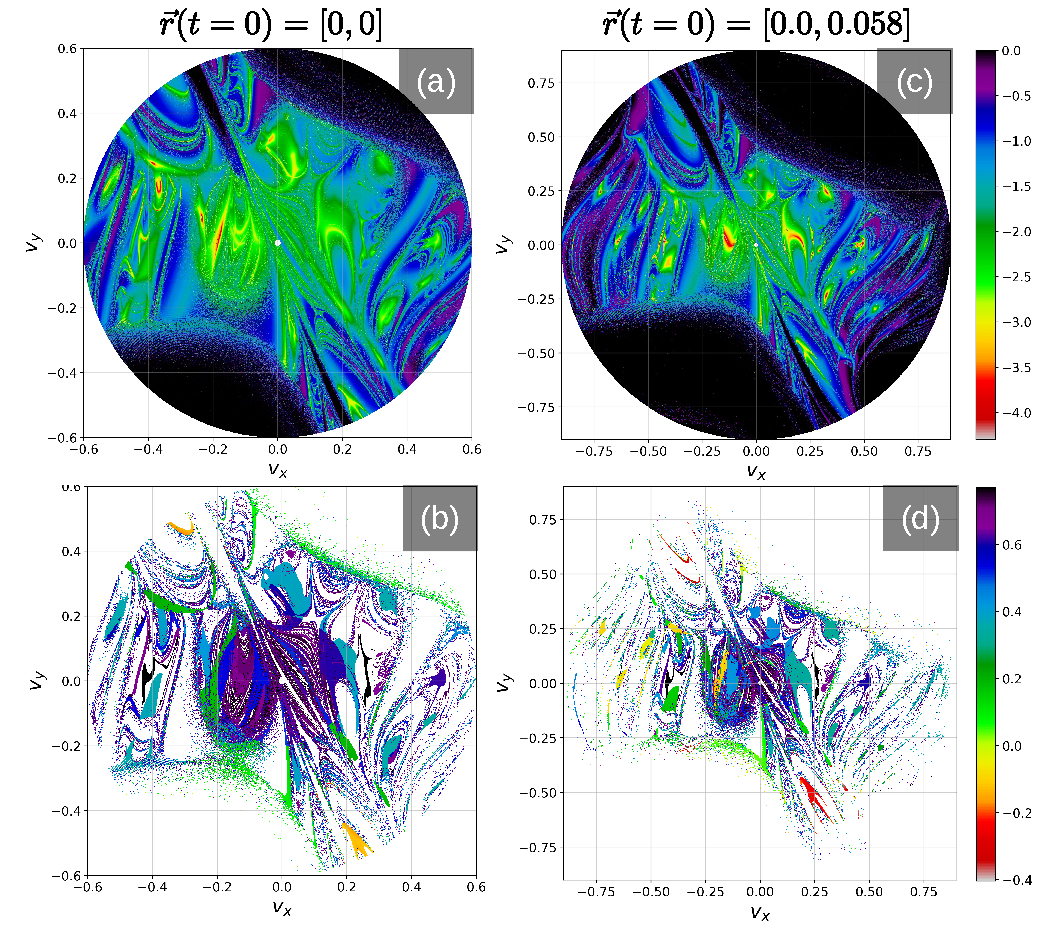
\includegraphics[width=1\linewidth]{diagrams/orbitFractals/e-fractals}
		\caption{Each pixel in the above images represents an individual trajectory formed by the $v_x,v_y$ coordinates of that pixel serving as an initial condition. In plots (a,c), each pixel is colored according to the minimum value of $\delta$, which is the closest approach to the initial conditions in phase space. The colorbar shows the value of $\log_e \delta_\mathrm{min}$. Trajectories which are nearly bounded are warmer colored. The plots (b,d) are colored according to the time of this closest approach. Warmer colors represent a shorter orbital period. The color bars are displaying the value of $\log_e t_\mathrm{closest}$.}
		\label{fig:e-fractals}
	\end{figure}
	
	\begin{figure}
		\centering
		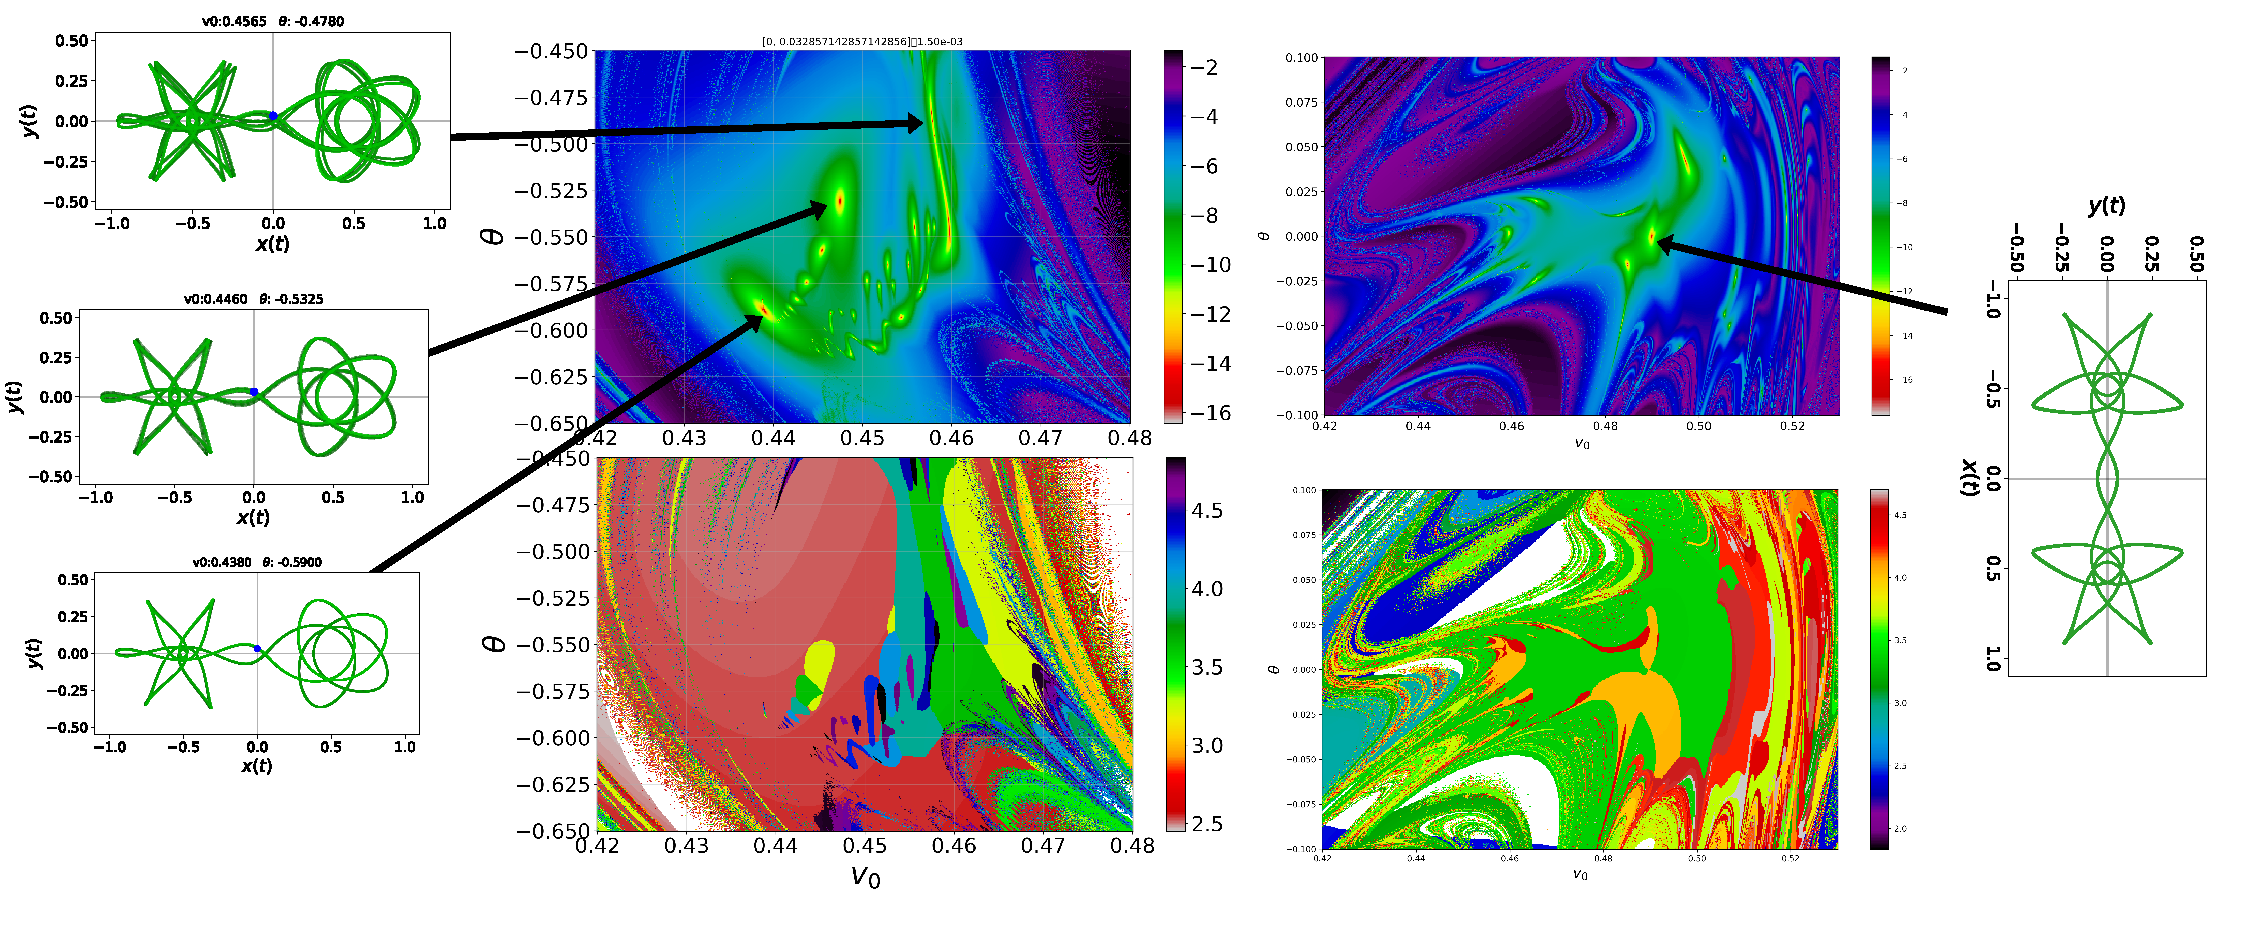
\includegraphics[width=1\linewidth]{diagrams/orbitFractals/orbitLegend}
		\caption{Orbits located within the phase diagram. Stable orbits can be located with the assistance of these color plots. Some of these points are the result of coincidence of the precession period with the orbital period. The upper plots are colored according to distance of closest approach in phase space. The lower plots are colored according to the time at this closest approach. Both color scales are logarithmic. The left two plots illustrate a region where asymmetric transfer orbits can be found. The region illustrated by the right plot contains the orbit specified by the initial conditions in the problem.}
		\label{fig:orbitlegend}
	\end{figure}
	
	\begin{figure}
		\centering
		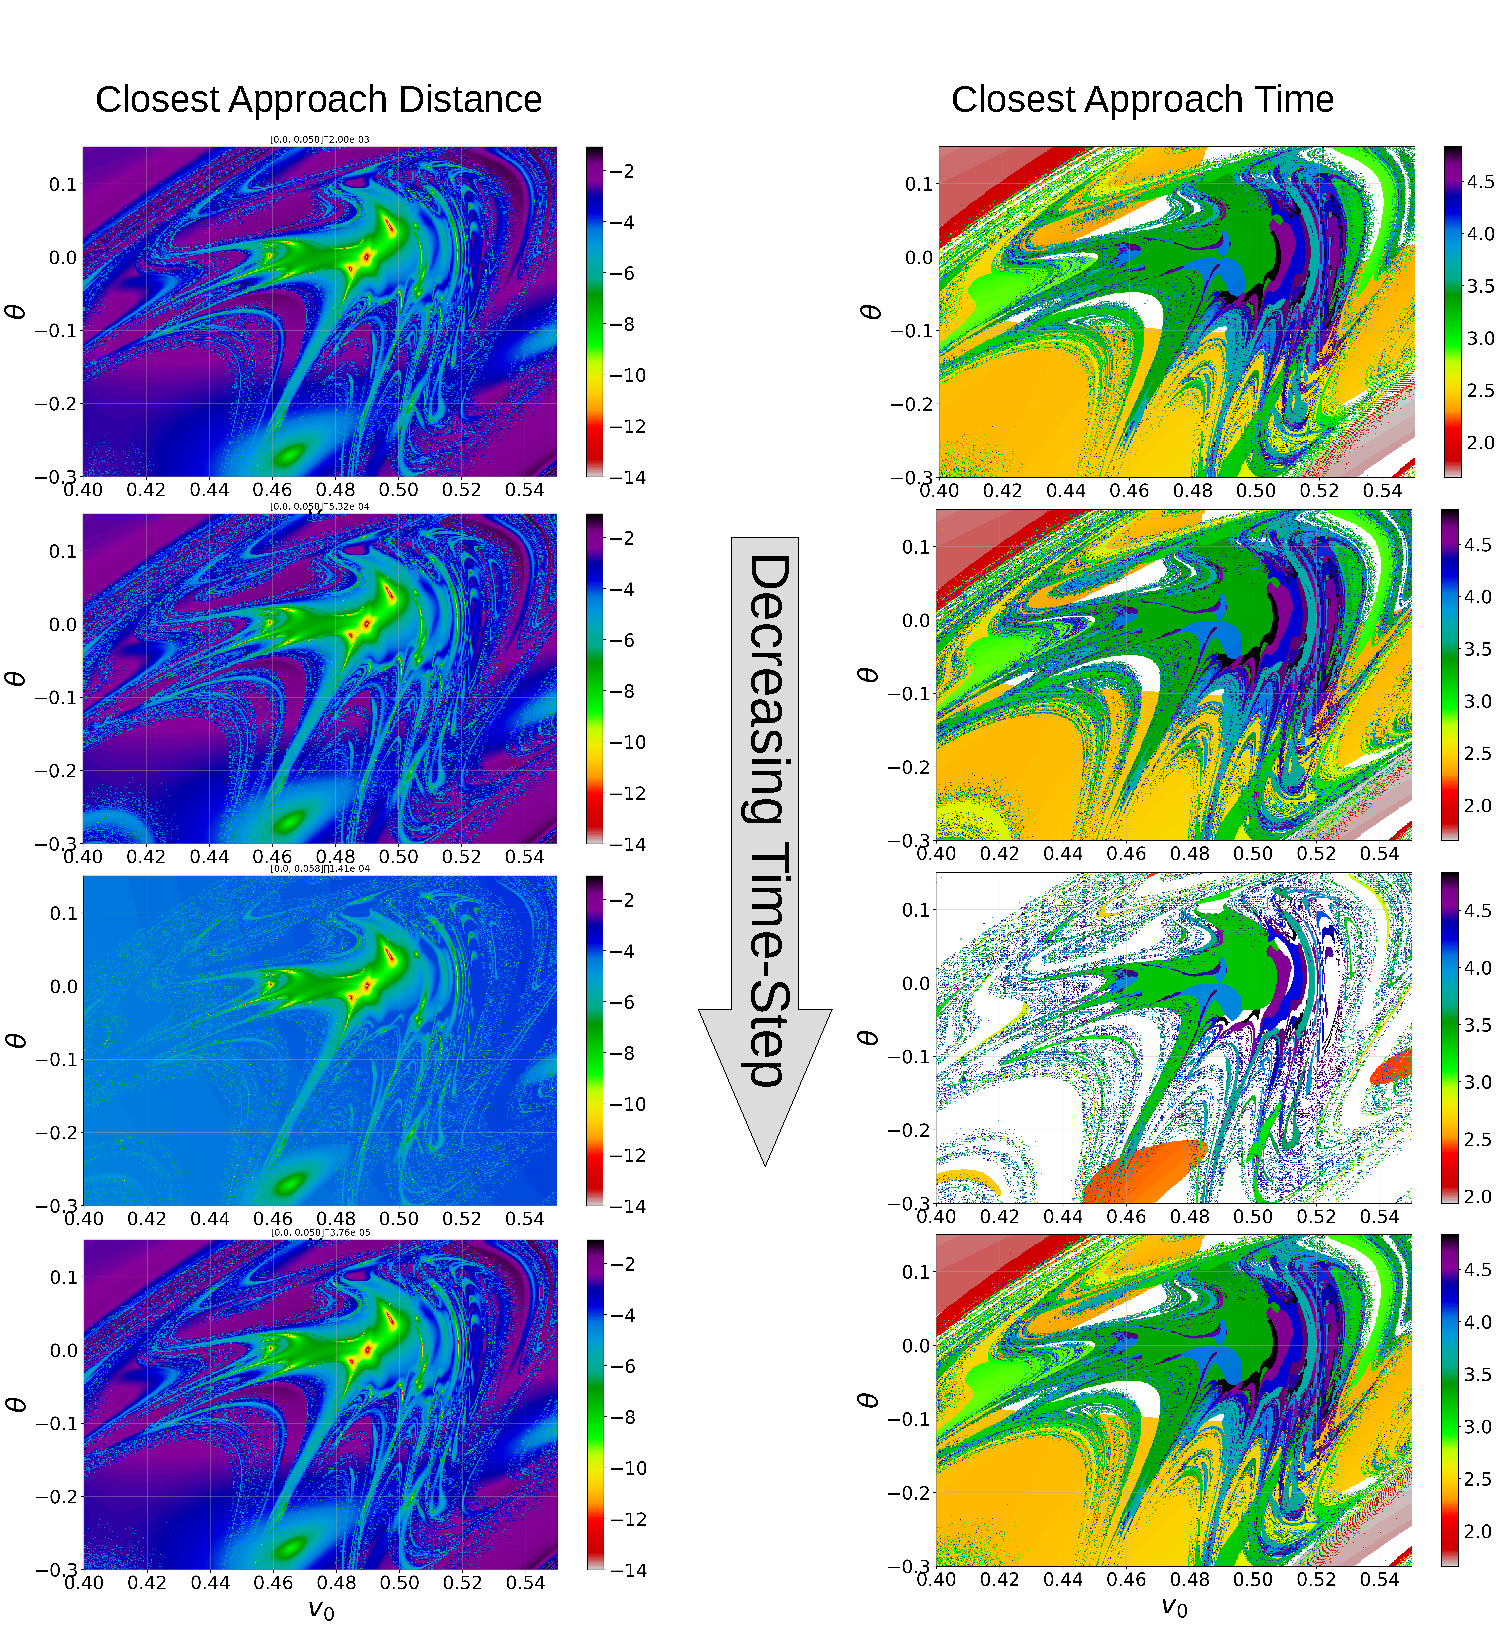
\includegraphics[width=1\linewidth]{diagrams/orbitFractals/f-decreasingTimeStep}
		\caption{Effect of decreasing time-step size. As the size of the time-step is decreased, more details in the diagram can be resolved. The fluctuation that occurs in the third row (from the top) is due to using a nearest point method for closest approach. This fluctuation can be improved by using interpolation of the trajectory points to find closest approach. This was not done in this work.}
		\label{fig:f-decreasingtimestep}
	\end{figure}
	
	\begin{figure}
		\centering
		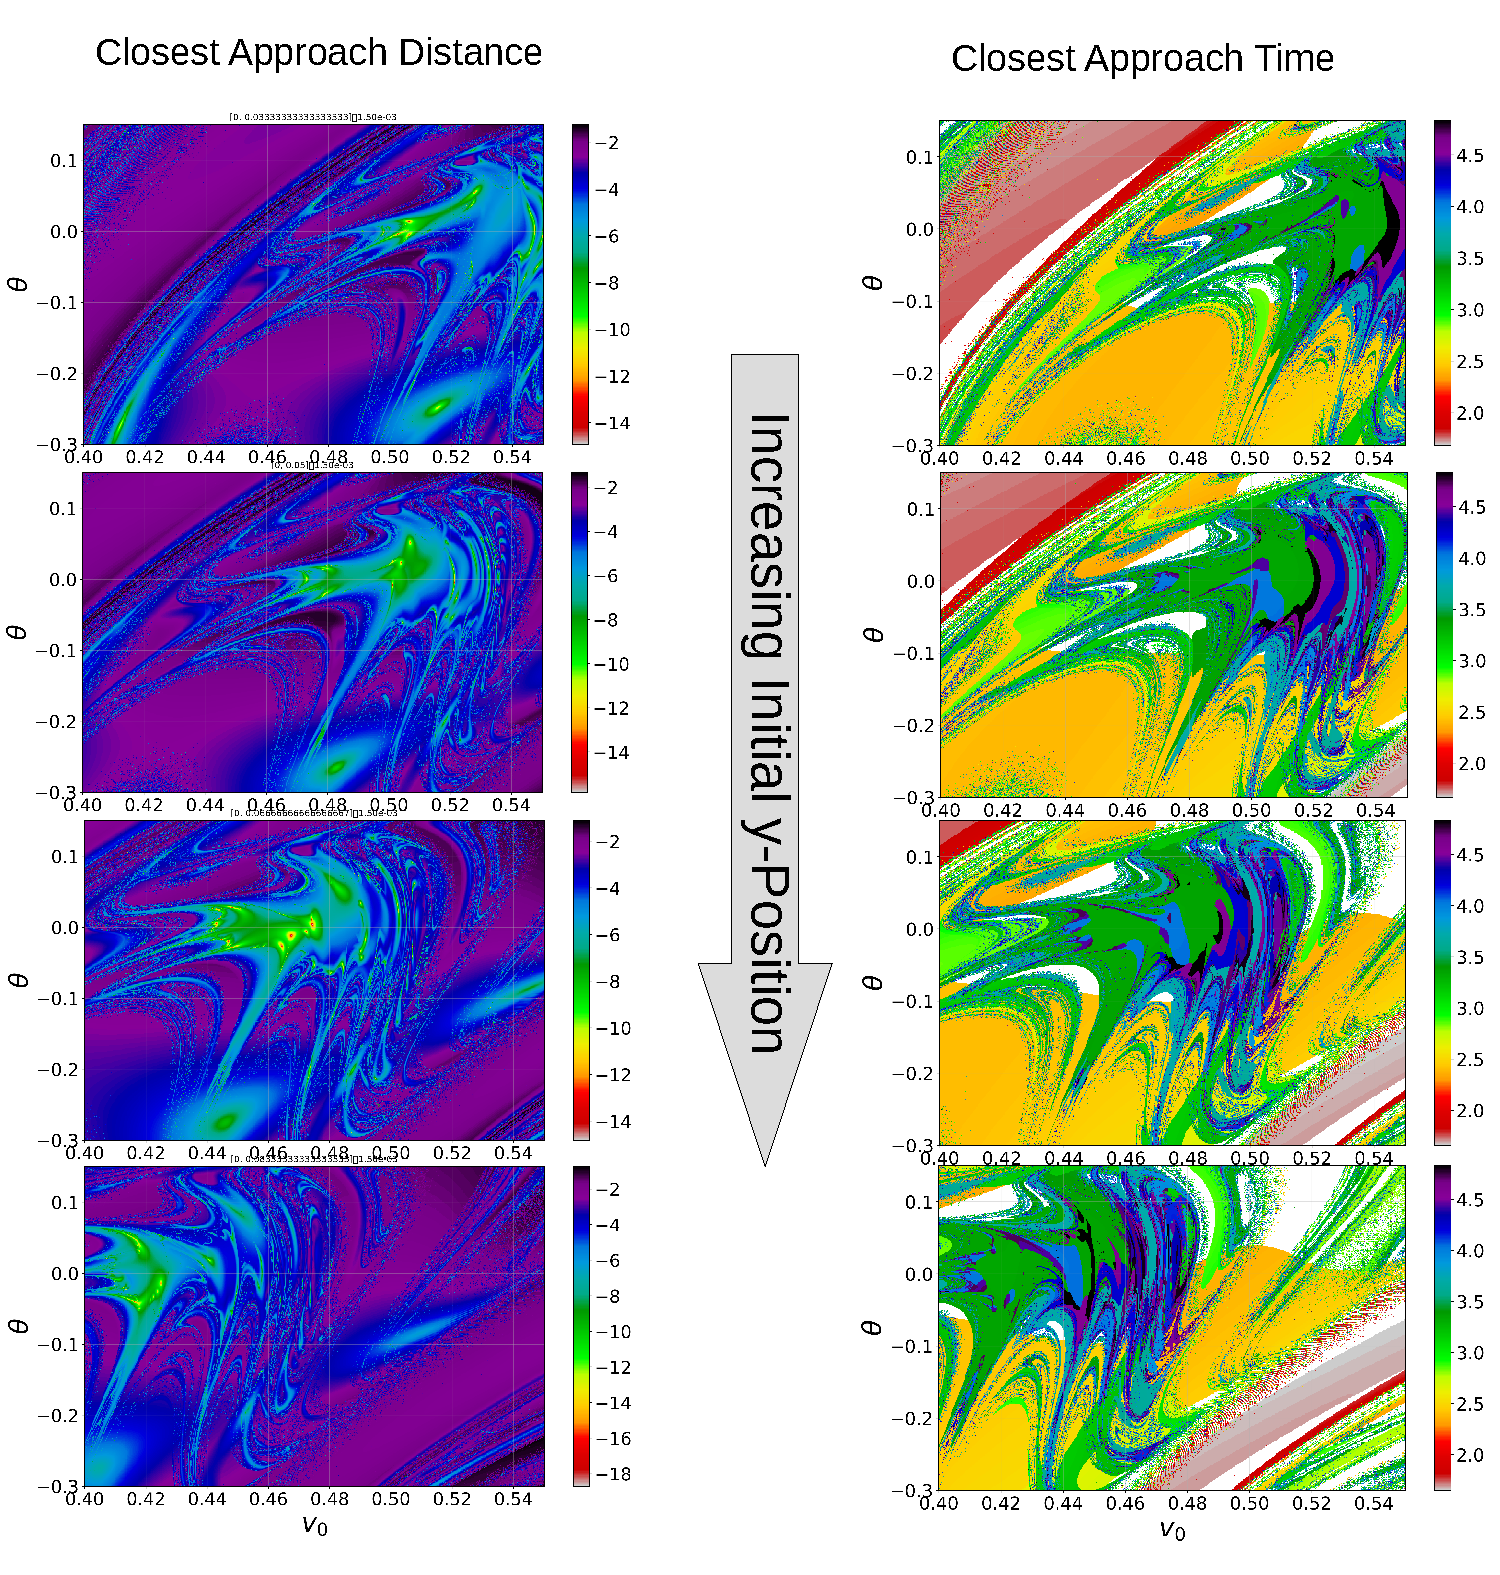
\includegraphics[width=1\linewidth]{diagrams/orbitFractals/f-changingY}
		\caption{Effect of changing initial position. As the initial position changes, the structure of the features evolves and shifts. The evolution of the plots as the initial position changes somewhat resembles a turbulent fluid. The left and right plots are depicting the same set of initial conditions, but the left plots are colored according to closest approach in phase space, and the right plots colored according to the time of this closest approach. }
		\label{fig:f-changingy}
	\end{figure}
	
\end{document}




